\documentclass[twoside]{book}

% Packages required by doxygen
\usepackage{fixltx2e}
\usepackage{calc}
\usepackage{doxygen}
\usepackage[export]{adjustbox} % also loads graphicx
\usepackage{graphicx}
\usepackage[utf8]{inputenc}
\usepackage{makeidx}
\usepackage{multicol}
\usepackage{multirow}
\PassOptionsToPackage{warn}{textcomp}
\usepackage{textcomp}
\usepackage[nointegrals]{wasysym}
\usepackage[table]{xcolor}

% Font selection
\usepackage[T1]{fontenc}
\usepackage[scaled=.90]{helvet}
\usepackage{courier}
\usepackage{amssymb}
\usepackage{sectsty}
\renewcommand{\familydefault}{\sfdefault}
\allsectionsfont{%
  \fontseries{bc}\selectfont%
  \color{darkgray}%
}
\renewcommand{\DoxyLabelFont}{%
  \fontseries{bc}\selectfont%
  \color{darkgray}%
}
\newcommand{\+}{\discretionary{\mbox{\scriptsize$\hookleftarrow$}}{}{}}

% Page & text layout
\usepackage{geometry}
\geometry{%
  a4paper,%
  top=2.5cm,%
  bottom=2.5cm,%
  left=2.5cm,%
  right=2.5cm%
}
\tolerance=750
\hfuzz=15pt
\hbadness=750
\setlength{\emergencystretch}{15pt}
\setlength{\parindent}{0cm}
\setlength{\parskip}{3ex plus 2ex minus 2ex}
\makeatletter
\renewcommand{\paragraph}{%
  \@startsection{paragraph}{4}{0ex}{-1.0ex}{1.0ex}{%
    \normalfont\normalsize\bfseries\SS@parafont%
  }%
}
\renewcommand{\subparagraph}{%
  \@startsection{subparagraph}{5}{0ex}{-1.0ex}{1.0ex}{%
    \normalfont\normalsize\bfseries\SS@subparafont%
  }%
}
\makeatother

% Headers & footers
\usepackage{fancyhdr}
\pagestyle{fancyplain}
\fancyhead[LE]{\fancyplain{}{\bfseries\thepage}}
\fancyhead[CE]{\fancyplain{}{}}
\fancyhead[RE]{\fancyplain{}{\bfseries\leftmark}}
\fancyhead[LO]{\fancyplain{}{\bfseries\rightmark}}
\fancyhead[CO]{\fancyplain{}{}}
\fancyhead[RO]{\fancyplain{}{\bfseries\thepage}}
\fancyfoot[LE]{\fancyplain{}{}}
\fancyfoot[CE]{\fancyplain{}{}}
\fancyfoot[RE]{\fancyplain{}{\bfseries\scriptsize Generated by Doxygen }}
\fancyfoot[LO]{\fancyplain{}{\bfseries\scriptsize Generated by Doxygen }}
\fancyfoot[CO]{\fancyplain{}{}}
\fancyfoot[RO]{\fancyplain{}{}}
\renewcommand{\footrulewidth}{0.4pt}
\renewcommand{\chaptermark}[1]{%
  \markboth{#1}{}%
}
\renewcommand{\sectionmark}[1]{%
  \markright{\thesection\ #1}%
}

% Indices & bibliography
\usepackage{natbib}
\usepackage[titles]{tocloft}
\setcounter{tocdepth}{3}
\setcounter{secnumdepth}{5}
\makeindex

% Hyperlinks (required, but should be loaded last)
\usepackage{ifpdf}
\ifpdf
  \usepackage[pdftex,pagebackref=true]{hyperref}
\else
  \usepackage[ps2pdf,pagebackref=true]{hyperref}
\fi
\hypersetup{%
  colorlinks=true,%
  linkcolor=blue,%
  citecolor=blue,%
  unicode%
}

% Custom commands
\newcommand{\clearemptydoublepage}{%
  \newpage{\pagestyle{empty}\cleardoublepage}%
}

\usepackage{caption}
\captionsetup{labelsep=space,justification=centering,font={bf},singlelinecheck=off,skip=4pt,position=top}

%===== C O N T E N T S =====

\begin{document}

% Titlepage & ToC
\hypersetup{pageanchor=false,
             bookmarksnumbered=true,
             pdfencoding=unicode
            }
\pagenumbering{alph}
\begin{titlepage}
\vspace*{7cm}
\begin{center}%
{\Large IR Laser Game \\[1ex]\large v1.\+0.\+1 }\\
\vspace*{1cm}
{\large Generated by Doxygen 1.8.14}\\
\end{center}
\end{titlepage}
\clearemptydoublepage
\pagenumbering{roman}
\tableofcontents
\clearemptydoublepage
\pagenumbering{arabic}
\hypersetup{pageanchor=true}

%--- Begin generated contents ---
\chapter{Hierarchical Index}
\section{Class Hierarchy}
This inheritance list is sorted roughly, but not completely, alphabetically\+:\begin{DoxyCompactList}
\item \contentsline{section}{Player}{\pageref{struct_player}}{}
\item task\begin{DoxyCompactList}
\item \contentsline{section}{display\+Task}{\pageref{classdisplay_task}}{}
\item \contentsline{section}{display\+Task}{\pageref{classdisplay_task}}{}
\item \contentsline{section}{game\+Time\+Control}{\pageref{classgame_time_control}}{}
\item \contentsline{section}{init\+Game}{\pageref{classinit_game}}{}
\item \contentsline{section}{ir\+\_\+decoder}{\pageref{classir__decoder}}{}
\item \contentsline{section}{ir\+\_\+receiver}{\pageref{classir__receiver}}{}
\item \contentsline{section}{ir\+\_\+transmitter}{\pageref{classir__transmitter}}{}
\item \contentsline{section}{keypad\+Task}{\pageref{classkeypad_task}}{}
\item \contentsline{section}{keypad\+Task}{\pageref{classkeypad_task}}{}
\item \contentsline{section}{main\+Game\+Control\+Task}{\pageref{classmain_game_control_task}}{}
\item \contentsline{section}{network\+Control}{\pageref{classnetwork_control}}{}
\item \contentsline{section}{register\+Game\+Control}{\pageref{classregister_game_control}}{}
\item \contentsline{section}{Trigger\+Task}{\pageref{class_trigger_task}}{}
\end{DoxyCompactList}
\item \contentsline{section}{Time}{\pageref{class_time}}{}
\item \contentsline{section}{Weapon}{\pageref{struct_weapon}}{}
\end{DoxyCompactList}

\chapter{Class Index}
\section{Class List}
Here are the classes, structs, unions and interfaces with brief descriptions\+:\begin{DoxyCompactList}
\item\contentsline{section}{\mbox{\hyperlink{classdisplay_task}{display\+Task}} \\*Display control }{\pageref{classdisplay_task}}{}
\item\contentsline{section}{\mbox{\hyperlink{classgame_time_control}{game\+Time\+Control}} }{\pageref{classgame_time_control}}{}
\item\contentsline{section}{\mbox{\hyperlink{classinit_game}{init\+Game}} }{\pageref{classinit_game}}{}
\item\contentsline{section}{\mbox{\hyperlink{classir__decoder}{ir\+\_\+decoder}} }{\pageref{classir__decoder}}{}
\item\contentsline{section}{\mbox{\hyperlink{classir__receiver}{ir\+\_\+receiver}} }{\pageref{classir__receiver}}{}
\item\contentsline{section}{\mbox{\hyperlink{classir__transmitter}{ir\+\_\+transmitter}} }{\pageref{classir__transmitter}}{}
\item\contentsline{section}{\mbox{\hyperlink{classkeypad_task}{keypad\+Task}} }{\pageref{classkeypad_task}}{}
\item\contentsline{section}{\mbox{\hyperlink{classmain_game_control_task}{main\+Game\+Control\+Task}} }{\pageref{classmain_game_control_task}}{}
\item\contentsline{section}{\mbox{\hyperlink{classnetwork_control}{network\+Control}} }{\pageref{classnetwork_control}}{}
\item\contentsline{section}{\mbox{\hyperlink{struct_player}{Player}} }{\pageref{struct_player}}{}
\item\contentsline{section}{\mbox{\hyperlink{classregister_game_control}{register\+Game\+Control}} }{\pageref{classregister_game_control}}{}
\item\contentsline{section}{\mbox{\hyperlink{class_time}{Time}} }{\pageref{class_time}}{}
\item\contentsline{section}{\mbox{\hyperlink{class_trigger_task}{Trigger\+Task}} }{\pageref{class_trigger_task}}{}
\item\contentsline{section}{\mbox{\hyperlink{struct_weapon}{Weapon}} }{\pageref{struct_weapon}}{}
\end{DoxyCompactList}

\chapter{Class Documentation}
\hypertarget{classdisplay_task}{}\section{display\+Task Class Reference}
\label{classdisplay_task}\index{display\+Task@{display\+Task}}


Display control.  




{\ttfamily \#include $<$display\+Task.\+hpp$>$}

Inheritance diagram for display\+Task\+:\begin{figure}[H]
\begin{center}
\leavevmode
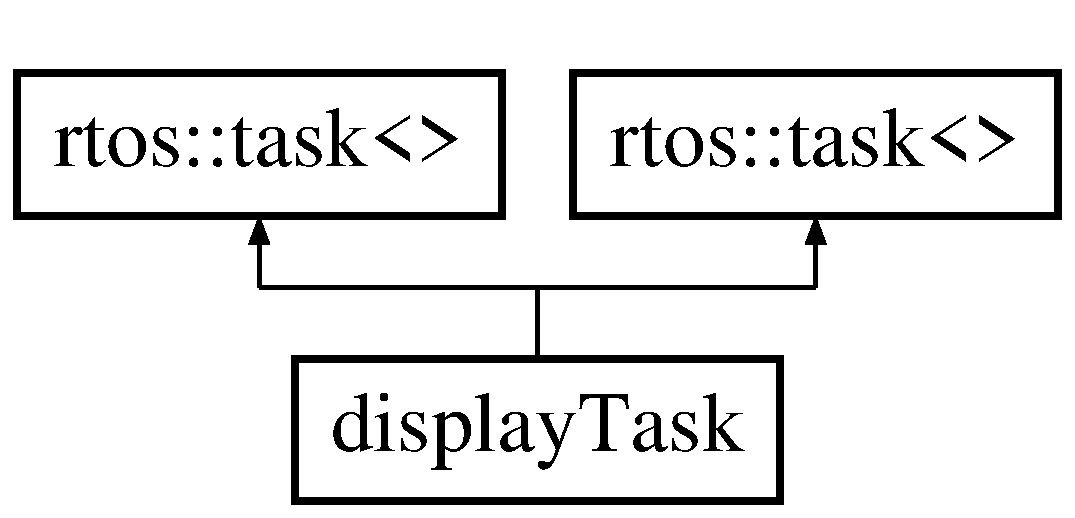
\includegraphics[height=2.000000cm]{classdisplay_task}
\end{center}
\end{figure}
\subsection*{Public Member Functions}
\begin{DoxyCompactItemize}
\item 
\mbox{\hyperlink{classdisplay_task_a6eaac17d19e3292654fb5c1bb952f5a7}{display\+Task}} (hwlib\+::window\+\_\+ostream \&display)
\begin{DoxyCompactList}\small\item\em \mbox{\hyperlink{classdisplay_task}{display\+Task}} constructor \end{DoxyCompactList}\item 
void \mbox{\hyperlink{classdisplay_task_a8197696b737d9ff890833e2dcf93b546}{main}} () override
\begin{DoxyCompactList}\small\item\em \mbox{\hyperlink{classdisplay_task}{display\+Task}}\textquotesingle{}s main method \end{DoxyCompactList}\item 
void \mbox{\hyperlink{classdisplay_task_a367b1904f141adf0817c16ad8fb1eb44}{show\+Game\+Time}} (const \mbox{\hyperlink{class_time}{Time}} \&t)
\begin{DoxyCompactList}\small\item\em Shows the current game time. \end{DoxyCompactList}\item 
void \mbox{\hyperlink{classdisplay_task_a8cbad9cd4eb7783c2619550bb5e9fe04}{show\+Ammo}} (const uint16\+\_\+t \&ammo)
\begin{DoxyCompactList}\small\item\em Shows the current ammunition. \end{DoxyCompactList}\item 
void \mbox{\hyperlink{classdisplay_task_adefc6996b2cd23e2996bd93ef10a0bb8}{show\+Weapon}} (hwlib\+::string$<$ 40 $>$ weapon)
\begin{DoxyCompactList}\small\item\em Shows the current weapon. \end{DoxyCompactList}\item 
void \mbox{\hyperlink{classdisplay_task_aa202bda76b1663f4be2b009fb358bd0f}{show\+Health}} (const uint16\+\_\+t \&hp)
\begin{DoxyCompactList}\small\item\em Shows current health. \end{DoxyCompactList}\item 
void \mbox{\hyperlink{classdisplay_task_acccd3bfbaa4ad2b4c93ad229da70c531}{show\+String}} (hwlib\+::string$<$ 40 $>$ msg)
\begin{DoxyCompactList}\small\item\em Shows a message. \end{DoxyCompactList}\item 
void \mbox{\hyperlink{classdisplay_task_a67990960198f75d5a9815dc4e5a9e375}{return\+Idle}} (void)
\begin{DoxyCompactList}\small\item\em Returns to idle state. \end{DoxyCompactList}\item 
void \mbox{\hyperlink{classdisplay_task_ab9aebca5a9d98bfb5c7fafe5b25ed2c4}{shot\+By}} (const uint16\+\_\+t \&player\+\_\+id, hwlib\+::string$<$ 40 $>$ w\+\_\+name)
\begin{DoxyCompactList}\small\item\em Shows who shot you. \end{DoxyCompactList}\item 
void \mbox{\hyperlink{classdisplay_task_ad34fd92a96e6aa1017db7a6af2ca2125}{show\+Choice}} (const int \&screen)
\begin{DoxyCompactList}\small\item\em Shows a choice menu. \end{DoxyCompactList}\item 
void \mbox{\hyperlink{classdisplay_task_ae47b5facd84033ed17a473e40d67e838}{set\+Number}} (const char \&number)
\begin{DoxyCompactList}\small\item\em Sets a number on the screen. \end{DoxyCompactList}\item 
\mbox{\Hypertarget{classdisplay_task_ac381d382075cc9257f2169e1338a2501}\label{classdisplay_task_ac381d382075cc9257f2169e1338a2501}} 
{\bfseries display\+Task} (hwlib\+::window\+\_\+ostream \&oled\+\_\+display)
\item 
\mbox{\Hypertarget{classdisplay_task_a08c7eab7bef446ebac2bc1653e4f1227}\label{classdisplay_task_a08c7eab7bef446ebac2bc1653e4f1227}} 
void {\bfseries main} ()
\item 
\mbox{\Hypertarget{classdisplay_task_a893409edcd5df80efc7f199c7cd9c697}\label{classdisplay_task_a893409edcd5df80efc7f199c7cd9c697}} 
void {\bfseries show\+Time} (const int \&t)
\item 
\mbox{\Hypertarget{classdisplay_task_a00a8fbd798e3b50ab4868ae288da296f}\label{classdisplay_task_a00a8fbd798e3b50ab4868ae288da296f}} 
void {\bfseries show\+Command} (const char \&c)
\item 
\mbox{\Hypertarget{classdisplay_task_a93807cbd6151cce058e3a86cb023a1e7}\label{classdisplay_task_a93807cbd6151cce058e3a86cb023a1e7}} 
void {\bfseries show\+State} (const int \&s)
\end{DoxyCompactItemize}


\subsection{Detailed Description}
Display control. 

This class implements the rtos\+::task$<$$>$ class and controls a 128x64 O\+L\+ED display. 

\subsection{Constructor \& Destructor Documentation}
\mbox{\Hypertarget{classdisplay_task_a6eaac17d19e3292654fb5c1bb952f5a7}\label{classdisplay_task_a6eaac17d19e3292654fb5c1bb952f5a7}} 
\index{display\+Task@{display\+Task}!display\+Task@{display\+Task}}
\index{display\+Task@{display\+Task}!display\+Task@{display\+Task}}
\subsubsection{\texorpdfstring{display\+Task()}{displayTask()}}
{\footnotesize\ttfamily display\+Task\+::display\+Task (\begin{DoxyParamCaption}\item[{hwlib\+::window\+\_\+ostream \&}]{display }\end{DoxyParamCaption})}



\mbox{\hyperlink{classdisplay_task}{display\+Task}} constructor 

This constructor requires a reference to a hwlib\+::window\+\_\+ostream object. 

\subsection{Member Function Documentation}
\mbox{\Hypertarget{classdisplay_task_a8197696b737d9ff890833e2dcf93b546}\label{classdisplay_task_a8197696b737d9ff890833e2dcf93b546}} 
\index{display\+Task@{display\+Task}!main@{main}}
\index{main@{main}!display\+Task@{display\+Task}}
\subsubsection{\texorpdfstring{main()}{main()}}
{\footnotesize\ttfamily void display\+Task\+::main (\begin{DoxyParamCaption}{ }\end{DoxyParamCaption})\hspace{0.3cm}{\ttfamily [override]}}



\mbox{\hyperlink{classdisplay_task}{display\+Task}}\textquotesingle{}s main method 

This method implements the rtos\+::task$<$$>$ method. \mbox{\Hypertarget{classdisplay_task_a67990960198f75d5a9815dc4e5a9e375}\label{classdisplay_task_a67990960198f75d5a9815dc4e5a9e375}} 
\index{display\+Task@{display\+Task}!return\+Idle@{return\+Idle}}
\index{return\+Idle@{return\+Idle}!display\+Task@{display\+Task}}
\subsubsection{\texorpdfstring{return\+Idle()}{returnIdle()}}
{\footnotesize\ttfamily void display\+Task\+::return\+Idle (\begin{DoxyParamCaption}\item[{void}]{ }\end{DoxyParamCaption})}



Returns to idle state. 

This function is used to return to the idle state. Use this method in combination with show\+String. \mbox{\Hypertarget{classdisplay_task_ae47b5facd84033ed17a473e40d67e838}\label{classdisplay_task_ae47b5facd84033ed17a473e40d67e838}} 
\index{display\+Task@{display\+Task}!set\+Number@{set\+Number}}
\index{set\+Number@{set\+Number}!display\+Task@{display\+Task}}
\subsubsection{\texorpdfstring{set\+Number()}{setNumber()}}
{\footnotesize\ttfamily void display\+Task\+::set\+Number (\begin{DoxyParamCaption}\item[{const char \&}]{number }\end{DoxyParamCaption})}



Sets a number on the screen. 

This method will show a number on the scree according to its parameters passed by. \mbox{\Hypertarget{classdisplay_task_ab9aebca5a9d98bfb5c7fafe5b25ed2c4}\label{classdisplay_task_ab9aebca5a9d98bfb5c7fafe5b25ed2c4}} 
\index{display\+Task@{display\+Task}!shot\+By@{shot\+By}}
\index{shot\+By@{shot\+By}!display\+Task@{display\+Task}}
\subsubsection{\texorpdfstring{shot\+By()}{shotBy()}}
{\footnotesize\ttfamily void display\+Task\+::shot\+By (\begin{DoxyParamCaption}\item[{const uint16\+\_\+t \&}]{player\+\_\+id,  }\item[{hwlib\+::string$<$ 40 $>$}]{w\+\_\+name }\end{DoxyParamCaption})}



Shows who shot you. 

This method shows who you were shot by, according to its parameters passed. \mbox{\Hypertarget{classdisplay_task_a8cbad9cd4eb7783c2619550bb5e9fe04}\label{classdisplay_task_a8cbad9cd4eb7783c2619550bb5e9fe04}} 
\index{display\+Task@{display\+Task}!show\+Ammo@{show\+Ammo}}
\index{show\+Ammo@{show\+Ammo}!display\+Task@{display\+Task}}
\subsubsection{\texorpdfstring{show\+Ammo()}{showAmmo()}}
{\footnotesize\ttfamily void display\+Task\+::show\+Ammo (\begin{DoxyParamCaption}\item[{const uint16\+\_\+t \&}]{ammo }\end{DoxyParamCaption})}



Shows the current ammunition. 

Shows the current ammunition according to its parameters passed. \mbox{\Hypertarget{classdisplay_task_ad34fd92a96e6aa1017db7a6af2ca2125}\label{classdisplay_task_ad34fd92a96e6aa1017db7a6af2ca2125}} 
\index{display\+Task@{display\+Task}!show\+Choice@{show\+Choice}}
\index{show\+Choice@{show\+Choice}!display\+Task@{display\+Task}}
\subsubsection{\texorpdfstring{show\+Choice()}{showChoice()}}
{\footnotesize\ttfamily void display\+Task\+::show\+Choice (\begin{DoxyParamCaption}\item[{const int \&}]{screen }\end{DoxyParamCaption})}



Shows a choice menu. 

Shows a choice menu according to which screen number is passed by. \mbox{\Hypertarget{classdisplay_task_a367b1904f141adf0817c16ad8fb1eb44}\label{classdisplay_task_a367b1904f141adf0817c16ad8fb1eb44}} 
\index{display\+Task@{display\+Task}!show\+Game\+Time@{show\+Game\+Time}}
\index{show\+Game\+Time@{show\+Game\+Time}!display\+Task@{display\+Task}}
\subsubsection{\texorpdfstring{show\+Game\+Time()}{showGameTime()}}
{\footnotesize\ttfamily void display\+Task\+::show\+Game\+Time (\begin{DoxyParamCaption}\item[{const \mbox{\hyperlink{class_time}{Time}} \&}]{t }\end{DoxyParamCaption})}



Shows the current game time. 

This method shows the current game time according to its parameters passed. \mbox{\Hypertarget{classdisplay_task_aa202bda76b1663f4be2b009fb358bd0f}\label{classdisplay_task_aa202bda76b1663f4be2b009fb358bd0f}} 
\index{display\+Task@{display\+Task}!show\+Health@{show\+Health}}
\index{show\+Health@{show\+Health}!display\+Task@{display\+Task}}
\subsubsection{\texorpdfstring{show\+Health()}{showHealth()}}
{\footnotesize\ttfamily void display\+Task\+::show\+Health (\begin{DoxyParamCaption}\item[{const uint16\+\_\+t \&}]{hp }\end{DoxyParamCaption})}



Shows current health. 

This method shows the current health according to its parameters passed. \mbox{\Hypertarget{classdisplay_task_acccd3bfbaa4ad2b4c93ad229da70c531}\label{classdisplay_task_acccd3bfbaa4ad2b4c93ad229da70c531}} 
\index{display\+Task@{display\+Task}!show\+String@{show\+String}}
\index{show\+String@{show\+String}!display\+Task@{display\+Task}}
\subsubsection{\texorpdfstring{show\+String()}{showString()}}
{\footnotesize\ttfamily void display\+Task\+::show\+String (\begin{DoxyParamCaption}\item[{hwlib\+::string$<$ 40 $>$}]{msg }\end{DoxyParamCaption})}



Shows a message. 

This method shows a string on the screen according to its parameters passed. \mbox{\Hypertarget{classdisplay_task_adefc6996b2cd23e2996bd93ef10a0bb8}\label{classdisplay_task_adefc6996b2cd23e2996bd93ef10a0bb8}} 
\index{display\+Task@{display\+Task}!show\+Weapon@{show\+Weapon}}
\index{show\+Weapon@{show\+Weapon}!display\+Task@{display\+Task}}
\subsubsection{\texorpdfstring{show\+Weapon()}{showWeapon()}}
{\footnotesize\ttfamily void display\+Task\+::show\+Weapon (\begin{DoxyParamCaption}\item[{hwlib\+::string$<$ 40 $>$}]{weapon }\end{DoxyParamCaption})}



Shows the current weapon. 

Shows the current weapon according to the parameters hwlib\+::string$<$40$>$ passed. 

The documentation for this class was generated from the following files\+:\begin{DoxyCompactItemize}
\item 
lasertag/display\+Task.\+hpp\item 
lasertag/display\+Task.\+cpp\end{DoxyCompactItemize}

\hypertarget{classgame_time_control}{}\section{game\+Time\+Control Class Reference}
\label{classgame_time_control}\index{game\+Time\+Control@{game\+Time\+Control}}
Inheritance diagram for game\+Time\+Control\+:\begin{figure}[H]
\begin{center}
\leavevmode
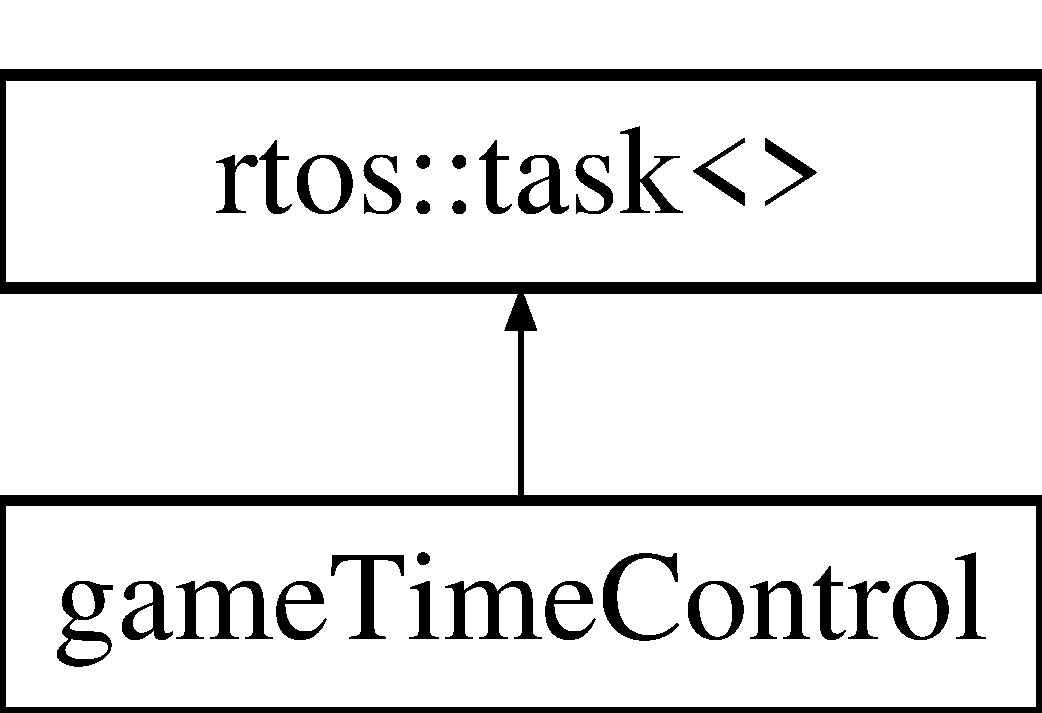
\includegraphics[height=2.000000cm]{classgame_time_control}
\end{center}
\end{figure}
\subsection*{Public Member Functions}
\begin{DoxyCompactItemize}
\item 
\mbox{\Hypertarget{classgame_time_control_a2401d43b6f5e68a806ff5190ddb2d307}\label{classgame_time_control_a2401d43b6f5e68a806ff5190ddb2d307}} 
{\bfseries game\+Time\+Control} (\mbox{\hyperlink{classdisplay_task}{display\+Task}} \&display)
\item 
\mbox{\Hypertarget{classgame_time_control_afb183d1589a21fdea5719cb266fb8abf}\label{classgame_time_control_afb183d1589a21fdea5719cb266fb8abf}} 
void {\bfseries set\+Time} (const \mbox{\hyperlink{class_time}{Time}} \&time)
\item 
\mbox{\Hypertarget{classgame_time_control_ac2f9139297b5a62c68378663e269ab90}\label{classgame_time_control_ac2f9139297b5a62c68378663e269ab90}} 
bool {\bfseries is\+Game\+Time\+Over} ()
\item 
\mbox{\Hypertarget{classgame_time_control_a21f29648cd0ac087aaa3ee278a4afef3}\label{classgame_time_control_a21f29648cd0ac087aaa3ee278a4afef3}} 
void {\bfseries start\+Game\+Timer} ()
\item 
\mbox{\Hypertarget{classgame_time_control_af81f8e6475d4ab3fdb8463013578d12d}\label{classgame_time_control_af81f8e6475d4ab3fdb8463013578d12d}} 
void {\bfseries main} () override
\end{DoxyCompactItemize}


The documentation for this class was generated from the following files\+:\begin{DoxyCompactItemize}
\item 
lasertag/game\+Time\+Control.\+hpp\item 
lasertag/game\+Time\+Control.\+cpp\end{DoxyCompactItemize}

\hypertarget{classinit_game}{}\section{init\+Game Class Reference}
\label{classinit_game}\index{init\+Game@{init\+Game}}
Inheritance diagram for init\+Game\+:\begin{figure}[H]
\begin{center}
\leavevmode
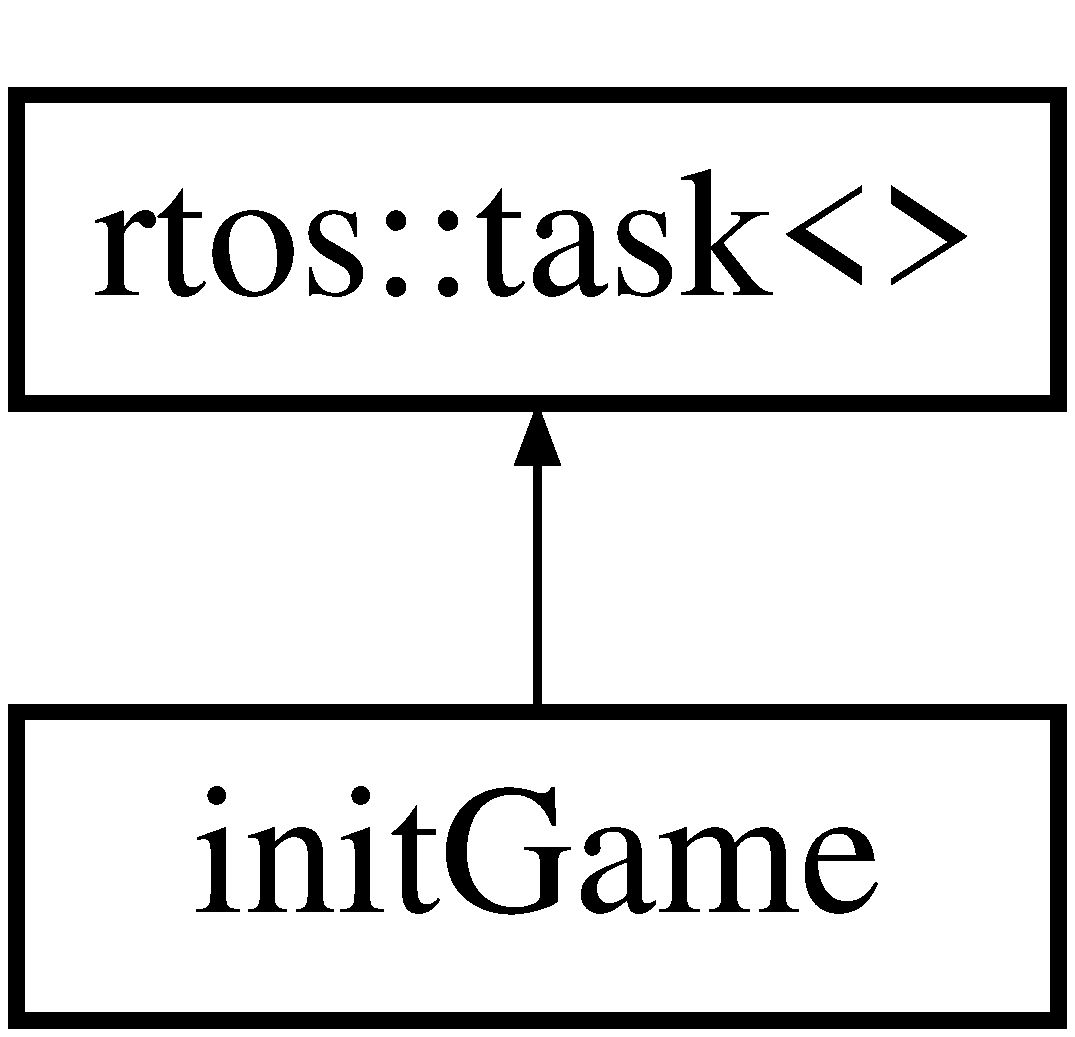
\includegraphics[height=2.000000cm]{classinit_game}
\end{center}
\end{figure}
\subsection*{Public Member Functions}
\begin{DoxyCompactItemize}
\item 
\mbox{\Hypertarget{classinit_game_af5c35bf90af47c83323a2202838ba88e}\label{classinit_game_af5c35bf90af47c83323a2202838ba88e}} 
{\bfseries init\+Game} (\mbox{\hyperlink{classdisplay_task}{display\+Task}} \&display\+Control, \mbox{\hyperlink{classir__transmitter}{ir\+\_\+transmitter}} \&transmitter\+Control)
\item 
\mbox{\Hypertarget{classinit_game_aaf342b77e471eeb385fbc966dc9cf467}\label{classinit_game_aaf342b77e471eeb385fbc966dc9cf467}} 
void {\bfseries button\+Pressed} (const char c)
\item 
\mbox{\Hypertarget{classinit_game_a94baf61c3957ffc14961f8bbdcf44a16}\label{classinit_game_a94baf61c3957ffc14961f8bbdcf44a16}} 
void {\bfseries main} ()
\end{DoxyCompactItemize}


The documentation for this class was generated from the following files\+:\begin{DoxyCompactItemize}
\item 
init\+Game/init\+Game.\+hpp\item 
init\+Game/init\+Game.\+cpp\end{DoxyCompactItemize}

\hypertarget{classir__decoder}{}\section{ir\+\_\+decoder Class Reference}
\label{classir__decoder}\index{ir\+\_\+decoder@{ir\+\_\+decoder}}
Inheritance diagram for ir\+\_\+decoder\+:\begin{figure}[H]
\begin{center}
\leavevmode
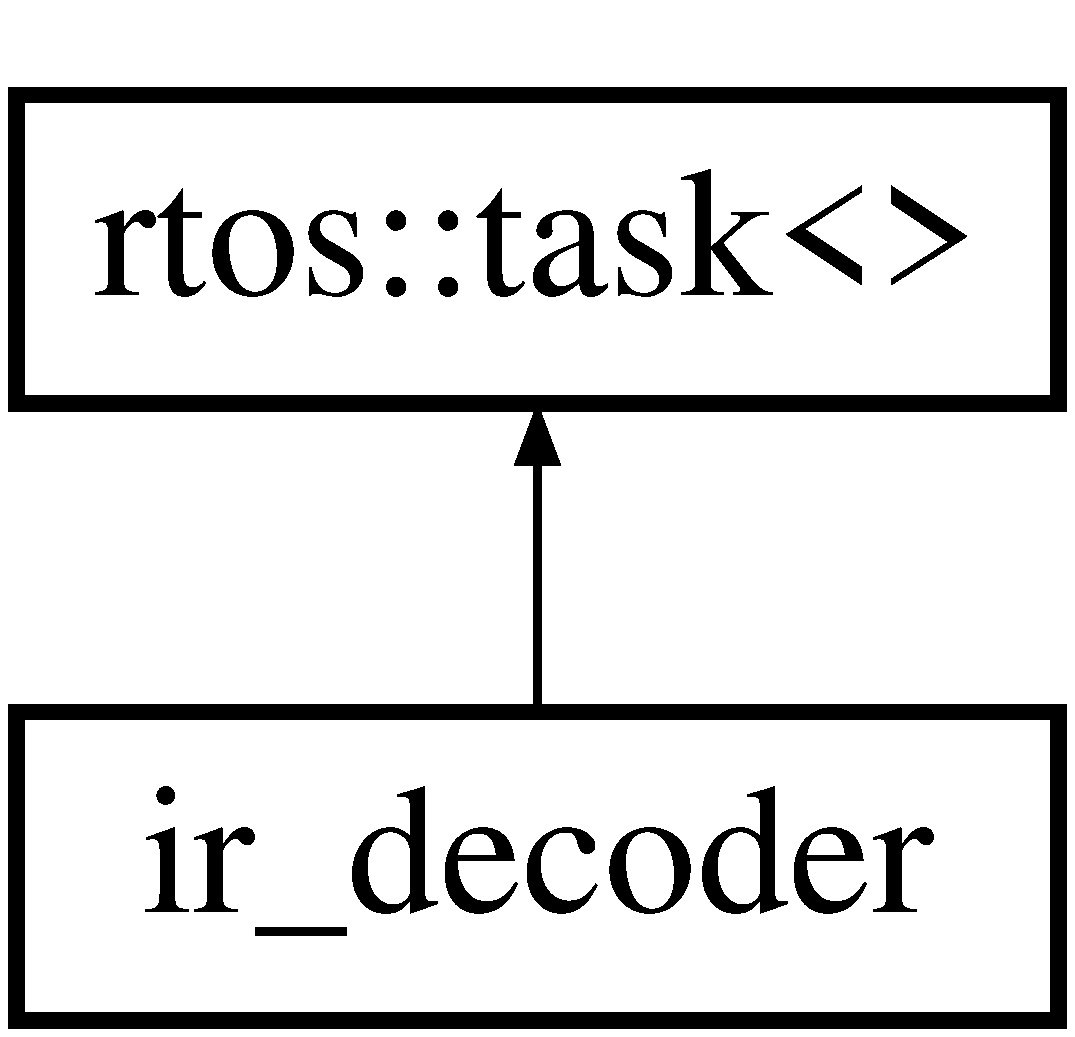
\includegraphics[height=2.000000cm]{classir__decoder}
\end{center}
\end{figure}
\subsection*{Public Member Functions}
\begin{DoxyCompactItemize}
\item 
\mbox{\Hypertarget{classir__decoder_a0a69c9508cf793ea50060666feece2f7}\label{classir__decoder_a0a69c9508cf793ea50060666feece2f7}} 
{\bfseries ir\+\_\+decoder} (\mbox{\hyperlink{classmain_game_control_task}{main\+Game\+Control\+Task}} \&main\+Game)
\item 
\mbox{\Hypertarget{classir__decoder_a84a8d41a1f2ea0bde2f90a997ab9e102}\label{classir__decoder_a84a8d41a1f2ea0bde2f90a997ab9e102}} 
void {\bfseries write\+\_\+message} (const int \&message1, const int \&message2)
\item 
\mbox{\Hypertarget{classir__decoder_adb89a214025bd79b5cb3a67cfd861956}\label{classir__decoder_adb89a214025bd79b5cb3a67cfd861956}} 
void {\bfseries main} () override
\end{DoxyCompactItemize}


The documentation for this class was generated from the following files\+:\begin{DoxyCompactItemize}
\item 
lasertag/ir\+\_\+decoder.\+hpp\item 
lasertag/ir\+\_\+decoder.\+cpp\end{DoxyCompactItemize}

\hypertarget{classir__receiver}{}\section{ir\+\_\+receiver Class Reference}
\label{classir__receiver}\index{ir\+\_\+receiver@{ir\+\_\+receiver}}
Inheritance diagram for ir\+\_\+receiver\+:\begin{figure}[H]
\begin{center}
\leavevmode
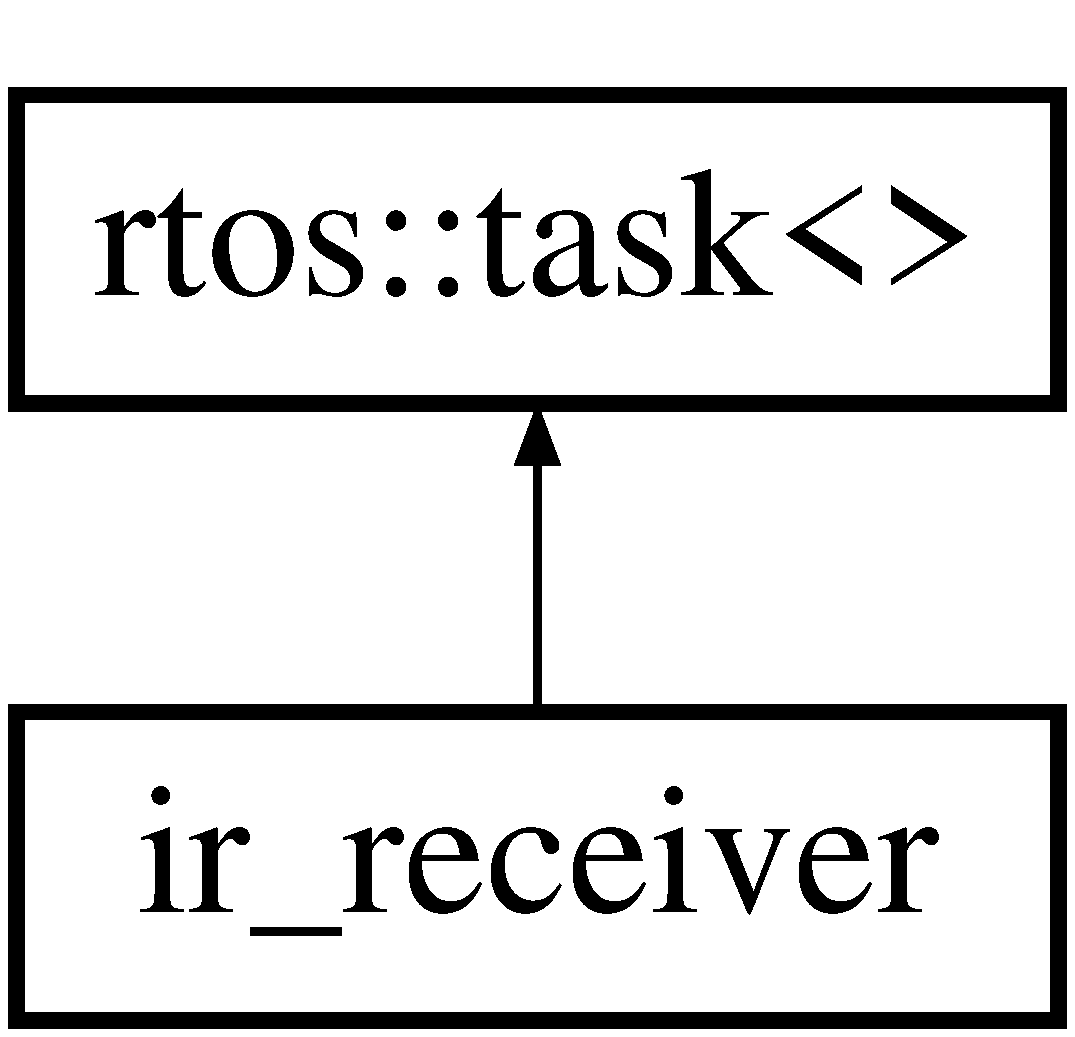
\includegraphics[height=2.000000cm]{classir__receiver}
\end{center}
\end{figure}
\subsection*{Public Member Functions}
\begin{DoxyCompactItemize}
\item 
\mbox{\Hypertarget{classir__receiver_a6dbdc36c8455ce5060a3f9e8357c1c57}\label{classir__receiver_a6dbdc36c8455ce5060a3f9e8357c1c57}} 
{\bfseries ir\+\_\+receiver} (hwlib\+::pin\+\_\+in \&receiver, \mbox{\hyperlink{classmain_game_control_task}{main\+Game\+Control\+Task}} \&main\+Game)
\item 
\mbox{\Hypertarget{classir__receiver_add394c4222f6c90fe9efc6603db578f0}\label{classir__receiver_add394c4222f6c90fe9efc6603db578f0}} 
void {\bfseries put\+Message} ()
\item 
\mbox{\Hypertarget{classir__receiver_a402529e38e6c904095a98525c57f9c25}\label{classir__receiver_a402529e38e6c904095a98525c57f9c25}} 
void {\bfseries main} () override
\end{DoxyCompactItemize}


The documentation for this class was generated from the following files\+:\begin{DoxyCompactItemize}
\item 
lasertag/ir\+\_\+receiver.\+hpp\item 
lasertag/ir\+\_\+receiver.\+cpp\end{DoxyCompactItemize}

\hypertarget{classir__transmitter}{}\section{ir\+\_\+transmitter Class Reference}
\label{classir__transmitter}\index{ir\+\_\+transmitter@{ir\+\_\+transmitter}}
Inheritance diagram for ir\+\_\+transmitter\+:\begin{figure}[H]
\begin{center}
\leavevmode
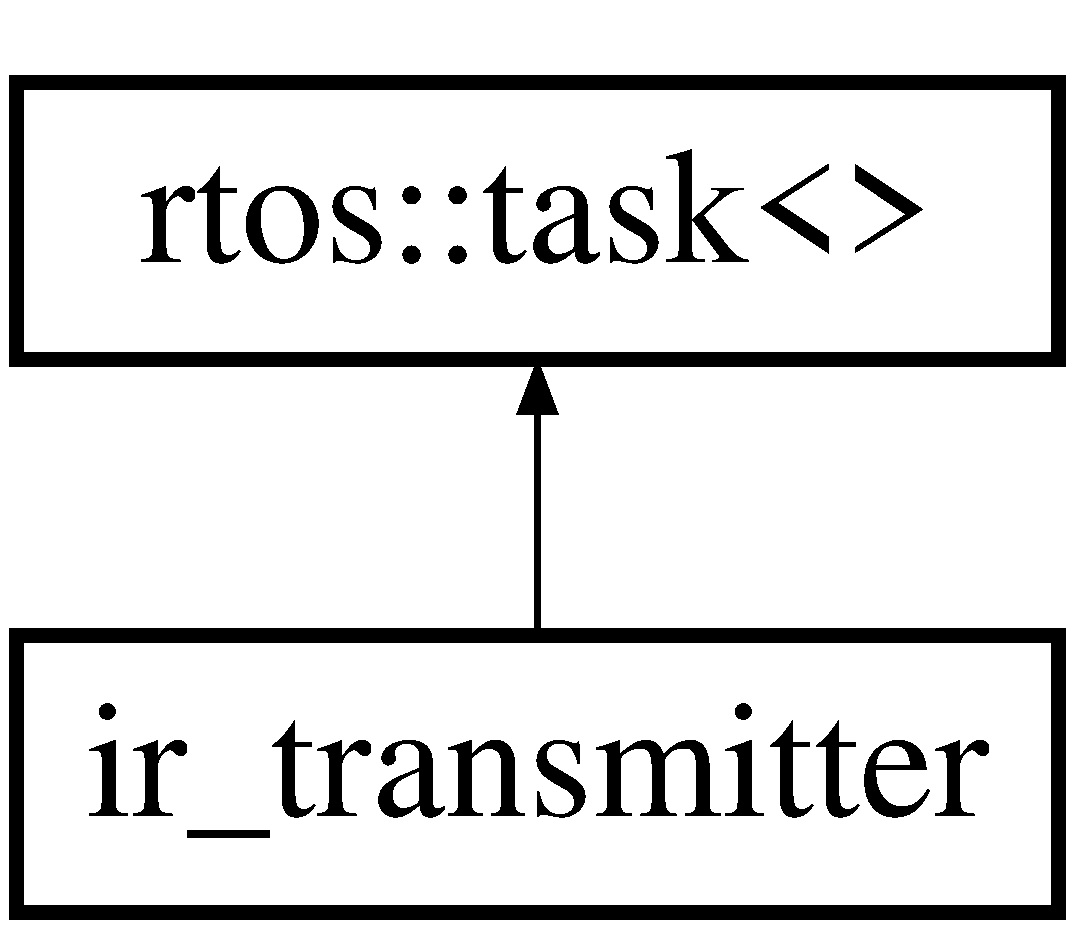
\includegraphics[height=2.000000cm]{classir__transmitter}
\end{center}
\end{figure}
\subsection*{Public Member Functions}
\begin{DoxyCompactItemize}
\item 
\mbox{\Hypertarget{classir__transmitter_a532f916d2330c2308558931e724a1418}\label{classir__transmitter_a532f916d2330c2308558931e724a1418}} 
{\bfseries ir\+\_\+transmitter} (hwlib\+::pin\+\_\+out \&transmitter)
\item 
\mbox{\Hypertarget{classir__transmitter_ae547c094efae5f733cb1d2291841450a}\label{classir__transmitter_ae547c094efae5f733cb1d2291841450a}} 
void {\bfseries send} (const uint16\+\_\+t \&player\+\_\+id, const uint16\+\_\+t \&data)
\item 
\mbox{\Hypertarget{classir__transmitter_a9dbedfe68066943a93ac4e109447e0a8}\label{classir__transmitter_a9dbedfe68066943a93ac4e109447e0a8}} 
void {\bfseries main} () override
\end{DoxyCompactItemize}


The documentation for this class was generated from the following files\+:\begin{DoxyCompactItemize}
\item 
lasertag/ir\+\_\+transmitter.\+hpp\item 
lasertag/ir\+\_\+transmitter.\+cpp\end{DoxyCompactItemize}

\hypertarget{classkeypad_task}{}\section{keypad\+Task Class Reference}
\label{classkeypad_task}\index{keypad\+Task@{keypad\+Task}}
Inheritance diagram for keypad\+Task\+:\begin{figure}[H]
\begin{center}
\leavevmode
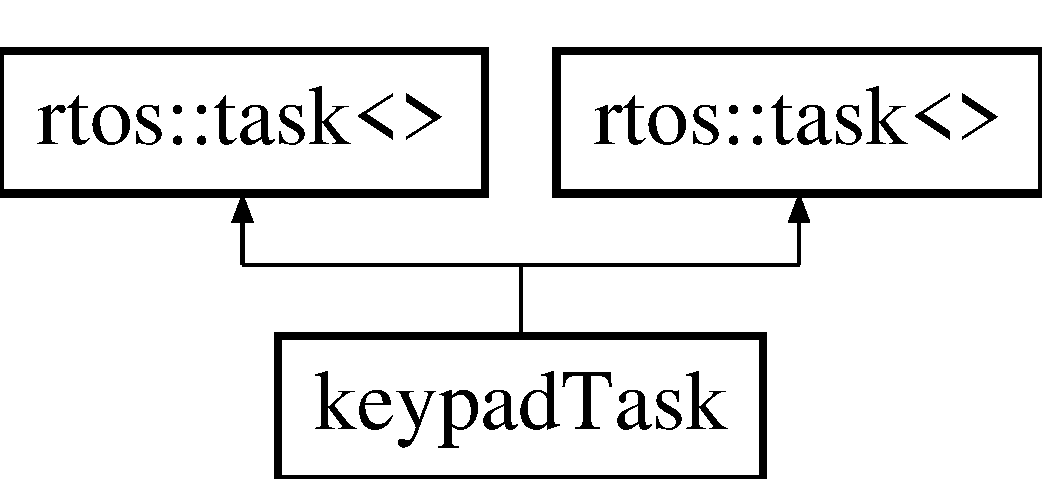
\includegraphics[height=2.000000cm]{classkeypad_task}
\end{center}
\end{figure}
\subsection*{Public Member Functions}
\begin{DoxyCompactItemize}
\item 
\mbox{\Hypertarget{classkeypad_task_acaa6c07951ed2676c09e6110ba6e3a80}\label{classkeypad_task_acaa6c07951ed2676c09e6110ba6e3a80}} 
{\bfseries keypad\+Task} (\mbox{\hyperlink{classregister_game_control}{register\+Game\+Control}} \&register\+Game)
\item 
\mbox{\Hypertarget{classkeypad_task_a32ea704ed454b4ecee6f805605133dd0}\label{classkeypad_task_a32ea704ed454b4ecee6f805605133dd0}} 
void {\bfseries main} ()
\item 
\mbox{\Hypertarget{classkeypad_task_ae4ff67f9cdad93df810036f66d3f22f5}\label{classkeypad_task_ae4ff67f9cdad93df810036f66d3f22f5}} 
{\bfseries keypad\+Task} (\mbox{\hyperlink{classinit_game}{init\+Game}} \&init\+Game\+Task)
\item 
\mbox{\Hypertarget{classkeypad_task_a32ea704ed454b4ecee6f805605133dd0}\label{classkeypad_task_a32ea704ed454b4ecee6f805605133dd0}} 
void {\bfseries main} ()
\end{DoxyCompactItemize}


The documentation for this class was generated from the following files\+:\begin{DoxyCompactItemize}
\item 
lasertag/keypad\+Task.\+hpp\item 
lasertag/keypad\+Task.\+cpp\end{DoxyCompactItemize}

\hypertarget{classmain_game_control_task}{}\section{main\+Game\+Control\+Task Class Reference}
\label{classmain_game_control_task}\index{main\+Game\+Control\+Task@{main\+Game\+Control\+Task}}
Inheritance diagram for main\+Game\+Control\+Task\+:\begin{figure}[H]
\begin{center}
\leavevmode
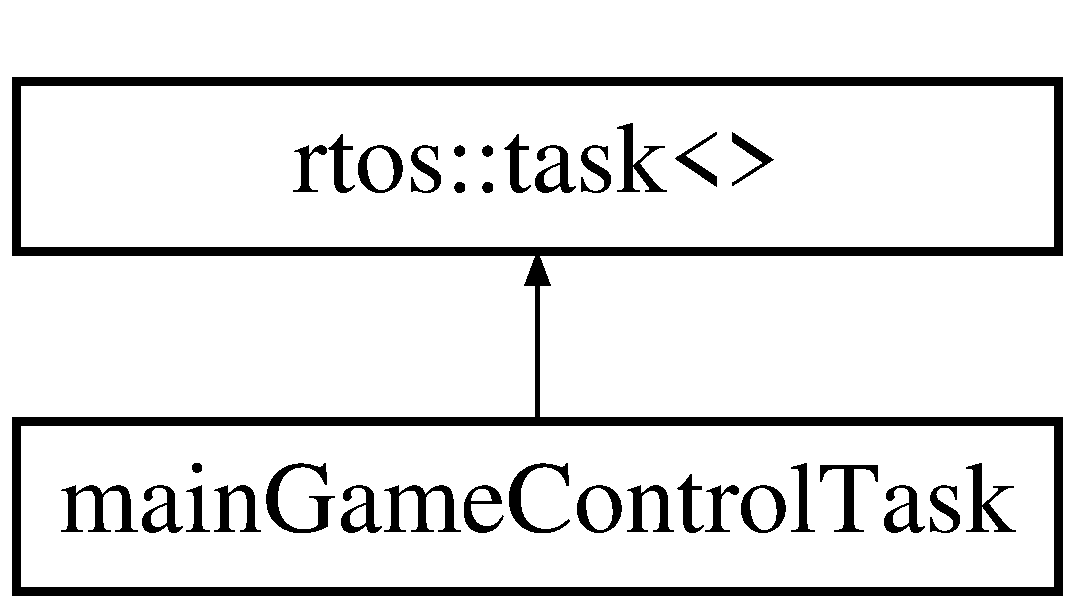
\includegraphics[height=2.000000cm]{classmain_game_control_task}
\end{center}
\end{figure}
\subsection*{Public Member Functions}
\begin{DoxyCompactItemize}
\item 
\mbox{\Hypertarget{classmain_game_control_task_a10dbf4428881f22899e385bd1f74991b}\label{classmain_game_control_task_a10dbf4428881f22899e385bd1f74991b}} 
{\bfseries main\+Game\+Control\+Task} (\mbox{\hyperlink{classir__transmitter}{ir\+\_\+transmitter}} \&transmitter, \mbox{\hyperlink{classdisplay_task}{display\+Task}} \&display, \mbox{\hyperlink{classgame_time_control}{game\+Time\+Control}} \&timer\+Control)
\item 
\mbox{\Hypertarget{classmain_game_control_task_a727395509964e10edf5323d7192c761b}\label{classmain_game_control_task_a727395509964e10edf5323d7192c761b}} 
void {\bfseries I\+R\+Message\+Received} (const uint16\+\_\+t \&player\+ID, const uint16\+\_\+t \&data)
\item 
\mbox{\Hypertarget{classmain_game_control_task_a7a04d0258e87093610ac8c8a73fed802}\label{classmain_game_control_task_a7a04d0258e87093610ac8c8a73fed802}} 
void {\bfseries triggered} ()
\item 
\mbox{\Hypertarget{classmain_game_control_task_a9044decbe55b509dc4d131734c5cb2ca}\label{classmain_game_control_task_a9044decbe55b509dc4d131734c5cb2ca}} 
void {\bfseries game\+Over} ()
\item 
\mbox{\Hypertarget{classmain_game_control_task_a727be41c2d7ae63c43f741cf59f8dcd3}\label{classmain_game_control_task_a727be41c2d7ae63c43f741cf59f8dcd3}} 
void {\bfseries set\+Player\+Params} (const uint16\+\_\+t \&player\+ID, const uint16\+\_\+t \&weapon\+ID)
\item 
\mbox{\Hypertarget{classmain_game_control_task_a9c2aeb99699a44c9d7bdea6f6aecfb96}\label{classmain_game_control_task_a9c2aeb99699a44c9d7bdea6f6aecfb96}} 
void {\bfseries main} () override
\end{DoxyCompactItemize}


The documentation for this class was generated from the following files\+:\begin{DoxyCompactItemize}
\item 
lasertag/main\+Game\+Control\+Task.\+hpp\item 
lasertag/main\+Game\+Control\+Task.\+cpp\end{DoxyCompactItemize}

\hypertarget{classnetwork_control}{}\section{network\+Control Class Reference}
\label{classnetwork_control}\index{network\+Control@{network\+Control}}
Inheritance diagram for network\+Control\+:\begin{figure}[H]
\begin{center}
\leavevmode
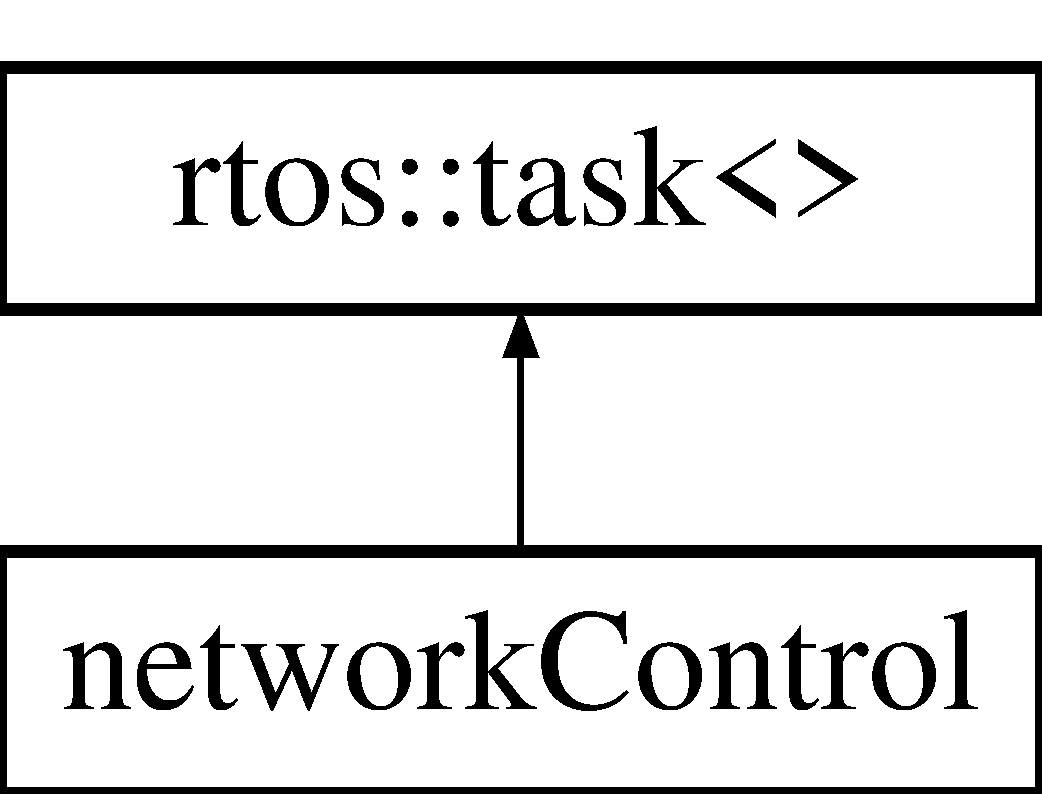
\includegraphics[height=2.000000cm]{classnetwork_control}
\end{center}
\end{figure}
\subsection*{Public Member Functions}
\begin{DoxyCompactItemize}
\item 
\mbox{\Hypertarget{classnetwork_control_ae4f1edf1741a10c22b9d45b1c440e71f}\label{classnetwork_control_ae4f1edf1741a10c22b9d45b1c440e71f}} 
{\bfseries network\+Control} (hwlib\+::pin\+\_\+out \&tx\+\_\+data, hwlib\+::pin\+\_\+out \&tx\+\_\+clock)
\item 
\mbox{\Hypertarget{classnetwork_control_a9aa41c3c526efd9c21ca95a47a5af39a}\label{classnetwork_control_a9aa41c3c526efd9c21ca95a47a5af39a}} 
void {\bfseries send\+Message} (const uint16\+\_\+t \&enemy\+Player\+Id, const uint16\+\_\+t \&weapon\+Damage)
\item 
\mbox{\Hypertarget{classnetwork_control_a8a562a0982afd0fe74b7140cf2fd6663}\label{classnetwork_control_a8a562a0982afd0fe74b7140cf2fd6663}} 
void {\bfseries main} () override
\end{DoxyCompactItemize}


The documentation for this class was generated from the following files\+:\begin{DoxyCompactItemize}
\item 
lasertag/network\+Control.\+hpp\item 
lasertag/network\+Control.\+cpp\end{DoxyCompactItemize}

\hypertarget{struct_player}{}\section{Player Struct Reference}
\label{struct_player}\index{Player@{Player}}
\subsection*{Public Attributes}
\begin{DoxyCompactItemize}
\item 
\mbox{\Hypertarget{struct_player_ae283754d5927f6442cd679e8b136e303}\label{struct_player_ae283754d5927f6442cd679e8b136e303}} 
uint16\+\_\+t {\bfseries p\+\_\+id} = 99
\item 
\mbox{\Hypertarget{struct_player_a71d61d40d49f9f9172253c1fafd97ba2}\label{struct_player_a71d61d40d49f9f9172253c1fafd97ba2}} 
uint16\+\_\+t {\bfseries hp} = 100
\item 
\mbox{\Hypertarget{struct_player_ad9cbb1b94a52f68782dd26b96eed169a}\label{struct_player_ad9cbb1b94a52f68782dd26b96eed169a}} 
uint16\+\_\+t {\bfseries shield} = 0
\item 
\mbox{\Hypertarget{struct_player_a8f977208d1212bf7dbd7c590017d9eb4}\label{struct_player_a8f977208d1212bf7dbd7c590017d9eb4}} 
uint16\+\_\+t {\bfseries score} = 0
\end{DoxyCompactItemize}


The documentation for this struct was generated from the following file\+:\begin{DoxyCompactItemize}
\item 
lasertag/player\+Data.\+hpp\end{DoxyCompactItemize}

\hypertarget{classregister_game_control}{}\section{register\+Game\+Control Class Reference}
\label{classregister_game_control}\index{register\+Game\+Control@{register\+Game\+Control}}
Inheritance diagram for register\+Game\+Control\+:\begin{figure}[H]
\begin{center}
\leavevmode
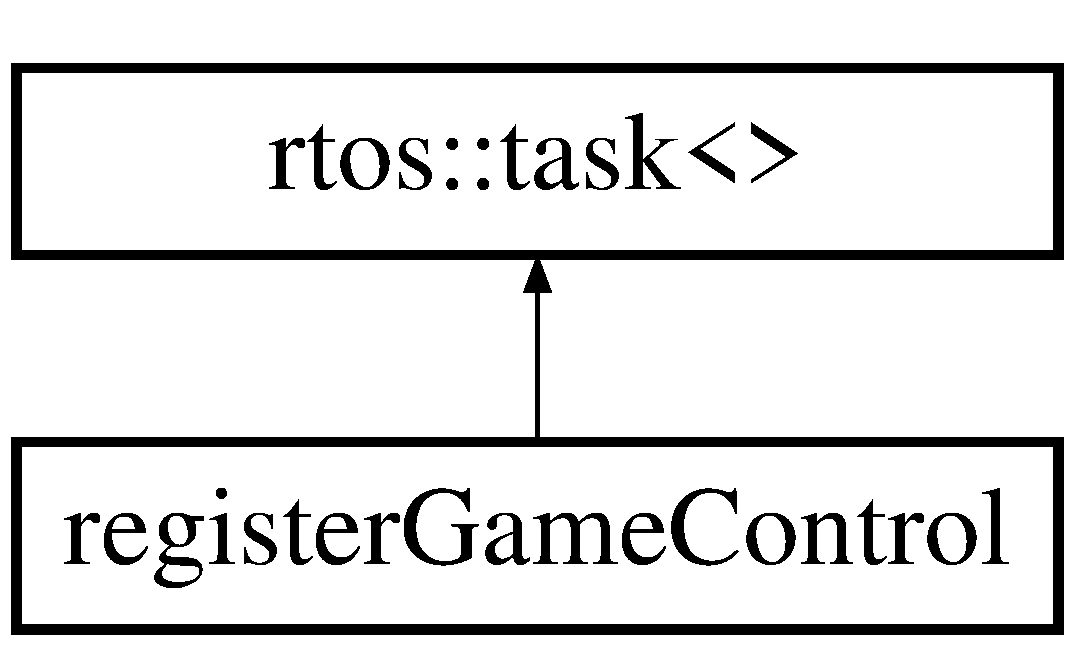
\includegraphics[height=2.000000cm]{classregister_game_control}
\end{center}
\end{figure}
\subsection*{Public Member Functions}
\begin{DoxyCompactItemize}
\item 
\mbox{\Hypertarget{classregister_game_control_a90674e16d0a4ec52c71b9e29a64ee003}\label{classregister_game_control_a90674e16d0a4ec52c71b9e29a64ee003}} 
{\bfseries register\+Game\+Control} (\mbox{\hyperlink{classmain_game_control_task}{main\+Game\+Control\+Task}} \&main\+Game, \mbox{\hyperlink{classdisplay_task}{display\+Task}} \&display)
\item 
\mbox{\Hypertarget{classregister_game_control_a36671245dcea8853ebcc88446b974929}\label{classregister_game_control_a36671245dcea8853ebcc88446b974929}} 
void {\bfseries button\+Pressed} (const char \&c)
\item 
\mbox{\Hypertarget{classregister_game_control_a4db3c71a142241827cc2e8444c25aeaa}\label{classregister_game_control_a4db3c71a142241827cc2e8444c25aeaa}} 
void {\bfseries main} ()
\end{DoxyCompactItemize}


The documentation for this class was generated from the following files\+:\begin{DoxyCompactItemize}
\item 
lasertag/register\+Game\+Control.\+hpp\item 
lasertag/register\+Game\+Control.\+cpp\end{DoxyCompactItemize}

\hypertarget{class_time}{}\section{Time Class Reference}
\label{class_time}\index{Time@{Time}}
\subsection*{Public Member Functions}
\begin{DoxyCompactItemize}
\item 
\mbox{\Hypertarget{class_time_aae2968f074ef2d14ef778891a22f39ee}\label{class_time_aae2968f074ef2d14ef778891a22f39ee}} 
{\bfseries Time} (const int \&min, const int \&sec)
\item 
\mbox{\Hypertarget{class_time_a93b57c132d115fc09e321072efee3cdc}\label{class_time_a93b57c132d115fc09e321072efee3cdc}} 
\mbox{\hyperlink{class_time}{Time}} {\bfseries get\+Time} () const
\item 
\mbox{\Hypertarget{class_time_afbc705df6c52b481418b559237a69a55}\label{class_time_afbc705df6c52b481418b559237a69a55}} 
int {\bfseries get\+Sec} () const
\item 
\mbox{\Hypertarget{class_time_a8cd37cf10b562d7f6efb418e7e0aa90a}\label{class_time_a8cd37cf10b562d7f6efb418e7e0aa90a}} 
int {\bfseries get\+Min} () const
\item 
\mbox{\Hypertarget{class_time_a6ca53f2e34d612ffb44e94b35186614b}\label{class_time_a6ca53f2e34d612ffb44e94b35186614b}} 
void {\bfseries update\+Time} ()
\end{DoxyCompactItemize}


The documentation for this class was generated from the following files\+:\begin{DoxyCompactItemize}
\item 
lasertag/time.\+hpp\item 
lasertag/time.\+cpp\end{DoxyCompactItemize}

\hypertarget{class_trigger_task}{}\section{Trigger\+Task Class Reference}
\label{class_trigger_task}\index{Trigger\+Task@{Trigger\+Task}}
Inheritance diagram for Trigger\+Task\+:\begin{figure}[H]
\begin{center}
\leavevmode
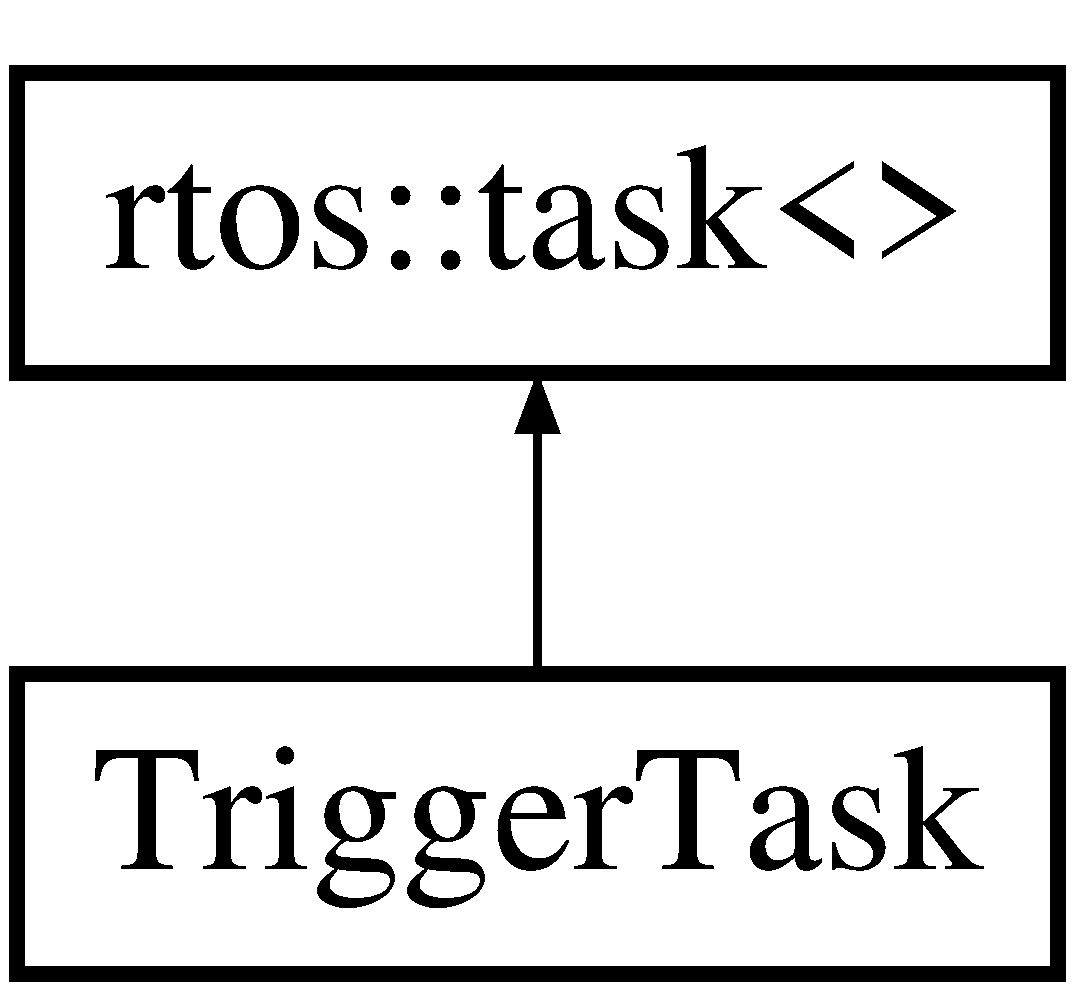
\includegraphics[height=2.000000cm]{class_trigger_task}
\end{center}
\end{figure}
\subsection*{Public Member Functions}
\begin{DoxyCompactItemize}
\item 
\mbox{\Hypertarget{class_trigger_task_a24b003a4ce868e75e35ff442c597c750}\label{class_trigger_task_a24b003a4ce868e75e35ff442c597c750}} 
{\bfseries Trigger\+Task} (hwlib\+::pin\+\_\+in \&trigger, \mbox{\hyperlink{classmain_game_control_task}{main\+Game\+Control\+Task}} \&main\+Game)
\item 
\mbox{\Hypertarget{class_trigger_task_a7a90964786348819cb2cf7e5a34cd69c}\label{class_trigger_task_a7a90964786348819cb2cf7e5a34cd69c}} 
void {\bfseries main} () override
\end{DoxyCompactItemize}


The documentation for this class was generated from the following files\+:\begin{DoxyCompactItemize}
\item 
lasertag/Trigger\+Task.\+hpp\item 
lasertag/Trigger\+Task.\+cpp\end{DoxyCompactItemize}

\hypertarget{struct_weapon}{}\section{Weapon Struct Reference}
\label{struct_weapon}\index{Weapon@{Weapon}}
\subsection*{Public Attributes}
\begin{DoxyCompactItemize}
\item 
\mbox{\Hypertarget{struct_weapon_a536ea9386102f7c456cee4a0b48a916b}\label{struct_weapon_a536ea9386102f7c456cee4a0b48a916b}} 
hwlib\+::string$<$ 40 $>$ {\bfseries name}
\item 
\mbox{\Hypertarget{struct_weapon_a66aef70c814827a6da3546d4ec754db2}\label{struct_weapon_a66aef70c814827a6da3546d4ec754db2}} 
uint16\+\_\+t {\bfseries damage}
\item 
\mbox{\Hypertarget{struct_weapon_a92136baff764c07f24bfac06706a3dc1}\label{struct_weapon_a92136baff764c07f24bfac06706a3dc1}} 
uint16\+\_\+t {\bfseries ammo}
\end{DoxyCompactItemize}


The documentation for this struct was generated from the following file\+:\begin{DoxyCompactItemize}
\item 
lasertag/player\+Data.\+hpp\end{DoxyCompactItemize}

%--- End generated contents ---

% Index
\backmatter
\newpage
\phantomsection
\clearemptydoublepage
\addcontentsline{toc}{chapter}{Index}
\printindex

\end{document}
